\documentclass{ctexart}
\usepackage{ctex}
\usepackage{graphicx}
\usepackage{mathtools}

\graphicspath{{figures/}}

\title{MatlabNotes}
\author{Mr Wu}
\date{\today}

\begin{document}
	\maketitle
	\section{基本操作}
	\subsection{变量}
	who,whos查看变量及变量类型;clc--清空命令行窗口;clear--清空工作区;
	
	特殊变量及常数:
	
	i,j:复数;inf:无穷;eps:很小的数;NaN:不是一个数
	
	查看matlab关键字:iskeyword
	
	不要用内嵌函数名和关键字名做为变量名字。matlab调用优先级:
	
	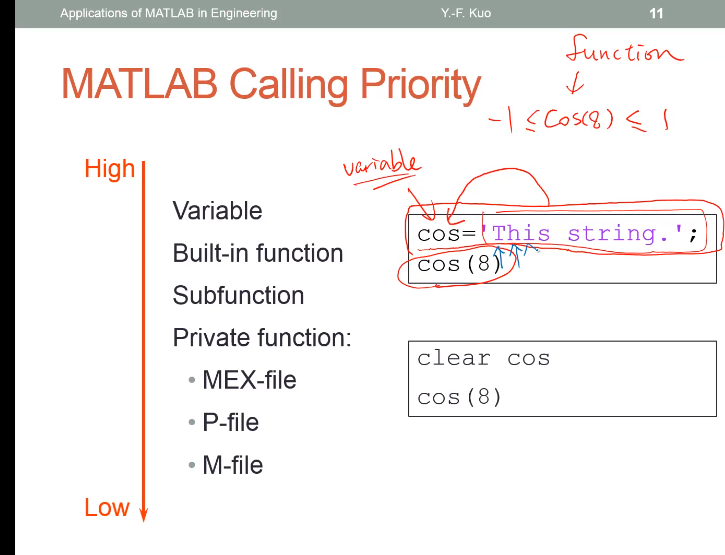
\includegraphics[scale=0.6]{1}
	
	\subsection{矩阵输入}
	输入行向量:a=[1 2 3 4]
	
	输入列向量:b=[1;2;3;4]
	
	输入矩阵:A=[1 2 3;4 5 6;7 8 9]
	
	\subsection{矩阵索引}
	A(i,j):i行j列元素
	
	A(i):一列一列数,第i个元素
	
	A([i j],[m n]):第i,j行和第m,n列的交叉元素,如A([1 3],[1,3])表示:
	
	$$ 
	\begin{bmatrix}
	1 & 3 \\
	7 & 9
	\end{bmatrix} $$
	
	\subsection{等差数列}
	C=[1:3:100]:定义一个数组,从1开始,100结束,即1,4,7,...,100.
	
	\subsection{删除矩阵的一行或一列}
	删除C的第二行:C(2,:)=[]
	
	\subsection{矩阵拼接}
	D=[A B];D=[A;B]
	
	\subsection{矩阵运算}
	$ A*B $: 普通的矩阵乘法
	
	$ A.*B $: element wise乘法,即对应元素相乘
	
	$ A/B $: A*inv(B)
	
	$ A./B $: element wise除法法,即对应元素相除
	
	$ A^a $: A的a次方
	
	$ A.^a $: A中每个元素变为自身的a次方
	
	\subsection{特殊矩阵}
	diag(v):以v中元素作为对角线元素的矩阵
	
	rand(m,n):mXn的正态分布的随机数
	
	\subsection{一些关于矩阵的函数}
	max(A): 返回矩阵中每一列最大的数组成的向量
	
	max(max(A)): 返回矩阵中最大的元素
	
	sum(A): 返回每一列元素的和组成的向量
	
	mean(A): 返回每一列元素的均值组成的向量
	\subsection{取整函数}
	Matlab取整函数有: fix, floor, ceil, round.具体应用方法如下:
	fix朝零方向取整,如fix(-1.3)=-1; fix(1.3)=1;
	floor,顾名思义,就是地板,所以是取比它小的整数,即朝负无穷方向取整,如floor(-1.3)=-2; floor(1.3)=1;floor(-1.8)=-2,floor(1.8)=1
	ceil,与floor相反,它的意思是天花板,也就是取比它大的最小整数,即朝正无穷方向取整,如ceil(-1.3)=-1; ceil(1.3)=2;ceil(-1.8)=-1,ceil(1.8)=2
	round四舍五入到最近的整数,如round(-1.3)=-1;round(-1.52)=-2;round(1.3)=1;round(1.52)=2。
	\section{自定义函数}
	1. 为变量预先分配空间可减少程序运行时间;
	
	2. function用法:
	
	定义:function [输出变量] = 函数名称(输入变量)
	
	调用:[输出变量] = 函数名(输入变量)
	
	3. ctrl+c可终止程序;
	
	4. 点乘,点除对应于输入变量是向量的情况;
	\section{变量}
	\subsection{rand函数}
	$ r=a+(b-a).*rand(100,1) $:生成$ (a,b) $区间之内的$ 100\times 1 $的随机数;
	
	$ r=randi(50,1,8) $:生成50以内的$ 1\times 8 $的随机数;
	\subsection{mean,var,std函数}
	1.mean(X):若X为矩阵,则计算每一列元素的均值,返回一个行向量。
	
	2.mean(X,dim):计算X第dim维上的均值。对于矩阵,列为第一维,行为第二维。
	
	3.mean2(X):计算矩阵X的均值。
	
	4.std(X,0,1):计算X列向量的标准差;std(X,0,2):计算X列向量的标准差。
	
	5.var(x):计算向量的方差。
	
	6.$ std(X,0,1).*std(X,0,1) $:计算X列向量的方差。
	\section{访问文件}
	
	
\end{document}